% TCP/IP vs. OSI: What’s the Difference Between the Two Models?
%   https://community.fs.com/blog/tcpip-vs-osi-whats-the-difference-between-the-two-models.html

\documentclass[tikz, border=10pt]{standalone}

\usepackage{tikz}
\usetikzlibrary{fit, positioning}
\newcommand{\fs}[1]{\fontsize{#1 pt}{0pt}\selectfont}
\usepackage{fontspec}
% \setmainfont{Calibri}
% \setmainfont{Cavorting}
% \setmainfont{Courgette}
\setmainfont{Doppio One}

\newcommand{\ys}{yshift}
\newcommand{\xs}{xshift}

\pgfdeclarelayer{bg}    % declare background layer
\pgfsetlayers{bg,main}  % set the order of the layers (main is the standard layer)

\begin{document}
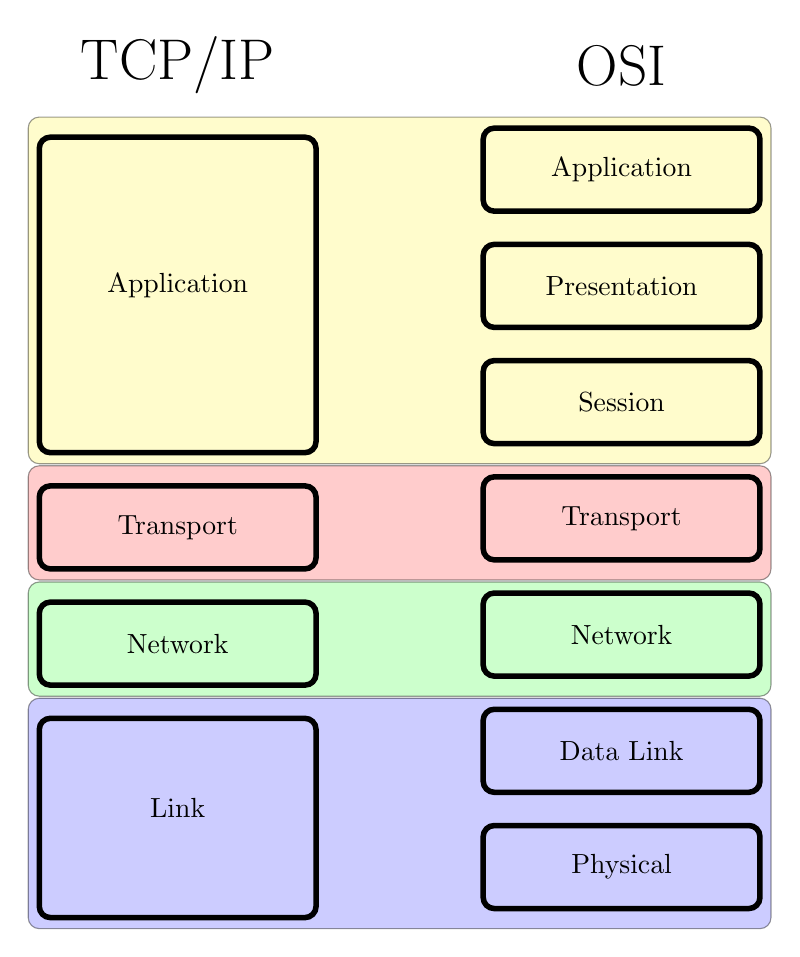
\begin{tikzpicture}[x=1pt,y=1pt]

\tikzstyle{title}=[font=\fs{20}, minimum width=100pt]
\tikzstyle{item}=[anchor=north, draw, line width=2pt, outer sep=0pt, inner sep=0pt, rounded corners, minimum width=100pt, minimum height=30pt, \ys=-12pt]

\node [title] (tcp) {TCP/IP};
% \node [title] (pro) [right,align=center] at ([xshift=20pt]tcp.east) {Protocols \& Services};
\node [title] (osi) [right] at ([xshift=60pt]tcp.east) {OSI};

\node [item] (osi1) at (osi.south) {Application};
\node [item] (osi2) at (osi1.south) {Presentation};
\node [item] (osi3) at (osi2.south) {Session};
\node [item] (osi4) at (osi3.south) {Transport};
\node [item] (osi5) at (osi4.south) {Network};
\node [item] (osi6) at (osi5.south) {Data Link};
\node [item] (osi7) at (osi6.south) {Physical};

\node [item, fit=(osi1)(osi2)(osi3), anchor=north] (tcp1) at (tcp.south) {Application};
\node [item] (tcp2) at (tcp1.south) {Transport};
\node [item] (tcp3) at (tcp2.south) {Network};
\node [item, fit=(osi6)(osi7), anchor=north] (tcp4) at (tcp3.south) {Link};

\begin{pgfonlayer}{bg}    % select the background layer
\node[fit=(osi1)(osi2)(osi3)(tcp1), draw, inner sep=4pt, rounded corners, fill=yellow!50, opacity=0.4] {};
\node[fit=(osi4)(tcp2), draw, inner sep=4pt, rounded corners, fill=red!50, opacity=0.4] {};
\node[fit=(osi5)(tcp3), draw, inner sep=4pt, rounded corners, fill=green!50, opacity=0.4] {};
\node[fit=(osi6)(osi7)(tcp4), draw, inner sep=4pt, rounded corners, fill=blue!50, opacity=0.4] {};
\end{pgfonlayer}

\end{tikzpicture}



\end{document}